\documentclass[12pt]{scrbook}

%\usepackage[a4paper, total={6in, 8in}]{geometry}

\usepackage{caption}
\usepackage{float}
\usepackage{hyperref}
\usepackage{graphicx}
\usepackage[nottoc, numbib]{tocbibind}
\usepackage{outlines}
\usepackage{listings}
\usepackage{minted}
\usepackage{paralist}

\KOMAoptions{twoside=false,parskip=half}

\setlength{\parindent}{0pt}

\RedeclareSectionCommands[
beforeskip=1em,
runin=false,
afterskip=-\parskip
]{paragraph,subparagraph}

\begin{document}

\author{Philipp Liermann 20-475873-20\\Supervisor: Prof. Dr. Raad Bin Tareaf}
\date{\today}

\title{ \begin{center} 
\includegraphics[width=8cm]{./images/logo.png}
	\end{center} \vspace{2cm} Hardening MFA web applications to counter evolving
	transparent phishing attack vectors \vspace{2cm} \large }

\maketitle

\newpage \tableofcontents

\newpage \chapter{Overview} \section{Abstract} As of today most online
services have implemented multi-factor authentication to prevent malicious
third-party actors from using stolen login credentials. Despite this, a new
technique referred to as transparent proxy phishing still provides malicious
actors the means of acquiring a victims private credentials and MFA tokens
during a classical social engineering based phishing attack. The attacker is
able to effectively duplicate legitimate services by using specifically
configured reverse proxy servers that relay traffic from the victims browser
to the original service while collecting and intercepting wanted information
like passwords and credit card numbers. Also the ease with which transparent
proxy phishing can be executed is alarming. Open-source toolkits and
publicly available resources have made it simpler than ever for attackers to
deploy such sophisticated schemes without a deep understanding of web
development or cybersecurity. This elevation in threat sophistication
underscores the urgent need for a corresponding advancement in defensive
measures. To resolve this issue, it is imperative to develop and implement
effective measures to counteract transparent phishing and alike. This paper
will review, evaluate and try to improve different strategies to help
developers protect their applications against this new type of phishing attack.

\newpage \section{Problem statement} As an online service provider
it is crucial to protect the privacy and security of its users. Due to the
fact that transparent or so called reverse proxy phishing attacks are
becoming more common and sophisticated implementing additional active
security measures to detect them is essential. The goal of this paper is to
provide a comprehensive overview of the current strategies to detect
transparent phishing attacks by watching incoming client traffic. As this
often requires TLS fingerprinting to detect known reverse proxy software the
paper will also try to propose a new approach of enumerating and actually
validating supported TLS ciphers of web browsers to make TLS fingerprint
spoofing harder for attackers.

\section{Research question}
This study centers on developing effective defenses for web applications against the rising threat of transparent proxy phishing attacks. The central question guiding this research is:
\begin{itemize}
    \item How can web applications be safeguarded against transparent proxy phishing attacks?
\end{itemize}
From this primary inquiry, several sub-questions emerge, focusing on specific aspects of the threat to better understand and address it:
\begin{itemize}
    \item What defines traditional phishing attacks, and how are they distinct from transparent proxy phishing attacks?

    This question aims to delineate the operational mechanisms of both, highlighting the unique challenges posed by the newer method.
    \item What is the magnitude of the threat posed by transparent proxy phishing attacks?

    Here, we seek to quantify the severity and prevalence of these attacks to better understand their impact on current security frameworks.
    \item How can a webserver detect that a client connection is being manipulated by a transparent phishing toolkit?

    This focuses on identifying the technical indicators that can alert servers to the presence of such phishing activities, forming the basis for developing more robust detection techniques.
\end{itemize}
These sub-questions are designed to dissect the broader problem into manageable segments, allowing for a more structured and focused inquiry into each aspect of transparent proxy phishing.

\section{Objective}
The objectives of this research are threefold. Firstly, it aims to elucidate the
mechanics and impact of transparent proxy phishing, underscoring why it is a
growing concern in the cybersecurity community. Secondly, the study evaluates
the current state of research, identifying gaps in existing defenses against
this attack vector. Finally, through rigorous experimentation and practical
simulations, the paper proposes new, effective strategies to mitigate this
threat, contributing valuable insights to the arsenal of cybersecurity defense
mechanisms.

\newpage \section{Theoretical foundations}
\paragraph{Cyberfraud} is a form of internet-based fraud, usually involving the
use of false identities and/or stolen information to illegally obtain money,
property, or services.
Cyberfraud is an increasingly pervasive problem that is becoming increasingly
difficult to combat, as fraudsters become more sophisticated in their methods.
In 2020, cyberfraud was estimated to cost the global economy over \$6
trillion\cite{6trillion}, with the financial sector suffering the most damages.
The social, economic and reputational costs of cyberfraud can be incredibly
damaging, and can range from the loss of money, to identity theft, to the
disruption of businesses. Cyberfraud has become so pervasive that it is
essential for businesses and individuals to take measures to protect themselves
from it. This includes using strong passwords and authentication systems that
require
two or even more external factors for authentication.

\paragraph{HTML} is the standard markup language for creating web pages
and web applications. It is used to structure and present content on the web.
HTML is used in conjunction with CSS and JavaScript to create interactive and
visually appealing web pages.

\paragraph{Unicode} is a standard for encoding,
representing, and handling text in most of the world's writing systems. It is
used to represent characters from all of the world's writing systems, including
Latin, Cyrillic, Greek, Arabic, Hebrew, Chinese, Japanese, Korean, and many
others. Unicode is used in many modern software applications, including web
browsers, word processors, and operating systems. In computer science
literature, Unicode symbols are often represented as U+ followed by a
hexadecimal number.

\paragraph{A Phishing attack} is a type of cyberattack in which an attacker
attempts to gain
confidential information, such as passwords, credit card numbers, or other
sensitive information, by sending emails or other messages disguised as
legitimate entities. These messages often include malicious links to faked login
prompts that will steal the victims credentials upon entering them. These
attacks are becoming increasingly sophisticated and difficult to recognize,
making it important for everyone to remain vigilant and take steps to protect
against them.

\paragraph{A HTTP reverse proxy} is a type of proxy server that
retrieves resources on behalf of a client from one or more servers. This type of
proxy is sometimes referred to as a “gateway” or “tunneling” proxy because it
acts as a gateway for the traffic to and from the server. A reverse proxy will
typically receive a request from a client, then forward that request to an
appropriate server on the same network. It then retrieves the response from the
server and sends it back to the client. This type of proxy server is most often
used in enterprise networks to protect against malicious traffic, to balance
load between multiple servers, and to cache static content.
\begin{figure}[!h]
	\centering
	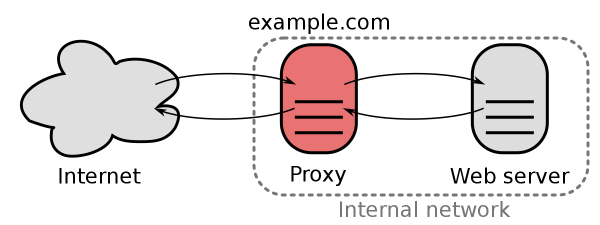
\includegraphics[height=4cm]{./images/http_reverse_proxy.png}
	\caption{How a HTTP reverse proxy works}
\end{figure}

\paragraph{Man in the Middle (MITM) attacks} are a type of
cyberattack in which an attacker intercepts and modifies communication between
two parties without their knowledge. This type of attack is often used to steal
sensitive information, such as login credentials, credit card numbers, or other
personal information. MITM attacks can be difficult to detect, as the attacker
can intercept and modify communication without the knowledge of the parties
involved.
\begin{figure}[!h] \centering
	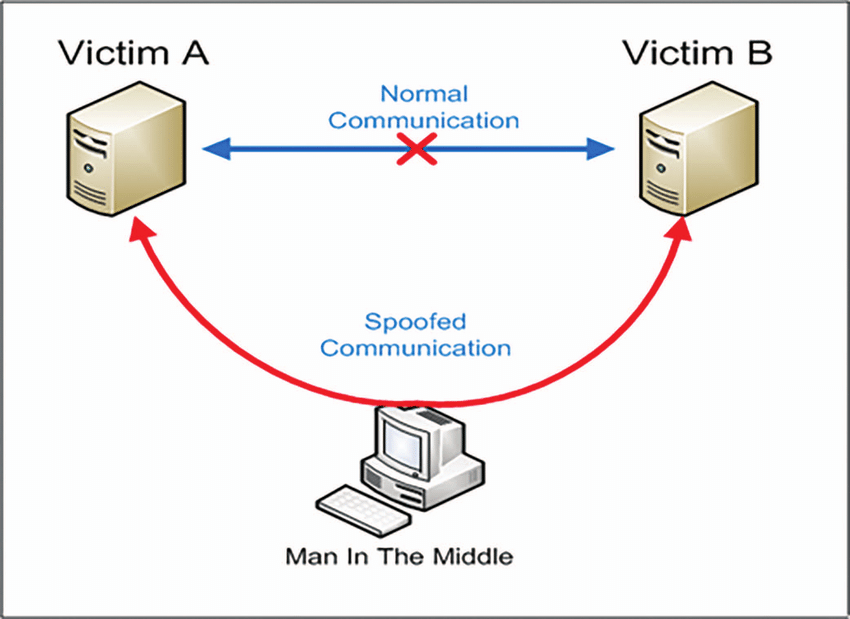
\includegraphics[height=6cm]{./images/mitm_attack.png}
	\caption{How a MITM attack works}
\end{figure}

\paragraph{Transparent proxy phishing} is a new technique used by attackers to
intercept and steal
multi-factor authentication (MFA) tokens from unsuspecting users. Instead of
copying HTML code from the original page that the attacker is trying to
impersonate, this new attack uses a HTTP reverse proxy to just redirect the
users traffic to the original page. The attacking proxy operator can view and
modify all traffic that is going through it while the victim sees a one by one
copy of the original login page. By doing so login credentials and 2FA tokens
can be extracted easily.

\paragraph{TLS} is a cryptographic protocol that provides
end-to-end security for data sent between a client and a server. It is widely
used to secure web traffic, email, and other types of data. TLS is the successor
to SSL, and is often referred to as SSL/TLS. If a webserver is using TLS its URL
starts with the well known https:// prefix.

\paragraph{TLS Fingerprinting} is a technique used to identify the TLS
implementation of a client or server by analyzing the handshake process. This
can be used to identify which software is
used by client or server. Industry standards for fingerprinting algorithms have
existed for a long time. These include: JA3, JA3N and the whole JA4+ family.

\paragraph{Nginx} is a popular open-source web server and reverse proxy server.
It is
used by millions of websites to serve web pages and other content. Nginx is
known for its high performance, stability, and low resource usage. It is also
known for its flexibility and extensibility, as it can be easily extended with
third-party modules and plugins. Because Nginx can easily be configured to act
as a reverse proxy and supports TLS, it is often used as a so called TLS
terminator, meaning that it terminates the TLS connection and forwards the
unencrypted traffic to a HTTP backend app.

\paragraph{Containerization}
is a lightweight alternative to full machine virtualization that involves
encapsulating an application in a container with its own operating environment.
Containers are isolated from one another and from the host system, but share the
same kernel. This makes them more lightweight and faster to start up than
virtual machines. Containers are often used to deploy applications in a
consistent and reproducible way, and are commonly used in cloud computing
environments.

\paragraph{Docker} is a platform for
developing, shipping, and running applications. It allows developers to package
their applications and dependencies into containers, which can then be run on
any system that has Docker installed. Docker containers are lightweight,
portable, and self-sufficient, making them an ideal platform for deploying
applications.

\paragraph{Podman} is a daemonless container engine for developing, managing,
and running OCI container images. It is very similar to Docker, but does not
require higher privileges to run containers as it fully runs in user space.

\paragraph{Socket} is an endpoint for communication between two machines or
processes. Sockets are used to establish a connection between a client and a
server, allowing them to exchange data. Sockets can be used to communicate over
a network or between processes on the same machine. On Linux hosts a socket can
even be represented as a file using the unix domain socket standard.

\paragraph{TCP} is a standard protocol that is used to establish and maintain a
connection between
two devices on a network. It is used to transmit data between devices in a
reliable and ordered manner. TCP is used in many applications, including web
servers,
email servers, and file transfer protocols. TCP is part of the TCP/IP protocol
suite.
A TCP connection is established using a three-way handshake, in which the client
and server
exchange a series of messages to establish a connection. These messages include
a SYN message
from the client, a SYN-ACK message from the server, and an ACK message from the
client.
Once the connection is established, data can be transmitted between the client
and server in both directions.

\paragraph{Wireshark} is a popular open-source network protocol
analyzer that is used to capture and analyze network traffic. It is widely used
by network administrators, security professionals, and developers to
troubleshoot network problems, analyze network traffic, and detect security
vulnerabilities.

\newpage \section{Current state of research}
The most prominent research on this topic is conducted in the paper
"Catching Transparent Phish: Analyzing and Detecting MITM Phishing Toolkits"
by Brian Kondracki Et al. \cite{kondracki2021catching}.
The team of four provides a detailed overview of the most used transparent
phishing toolkits and provides a list of statistical features that can be used to detect
those by testing the TLS server of the toolkit.
This list of features includes TLS fingerprints, User-Agents, simulated global
network delay and TCP packet timings from benchmarks of said tools.
Their model was able to detect the most common open-source MITM transparent
phishing toolkits with an accuracy above 99\%.
It is intended to be used with a script that scans the internet for phishing
sites that are run using MITM phishing toolkits.
Both is available as open-source on GitHub under the name PHOCA which means seal
in latin.\cite{kondracki2021catchingGit}
Through this research some of the chosen features for MITM toolkit server
detection will be used to watch client traffic for signs of it being relayed
through a transparent phishing toolkit.

Besides the research that has been done on this topic already, still we are far away from
production ready plug-n-play solutions that can reliably identify transparent phishing toolkits.

\section{Research Design}
First, a thorough analysis of existing and scientific papers on transparent
proxy
phishing toolkits will be undertaken. This literature review will critically
evaluate prior research findings, methodologies, and theoretical frameworks
deployed in the study of phishing attacks and defense mechanisms. By doing
so, it will identify potential gaps in the current body of knowledge and
establish
a solid theoretical foundation for subsequent experimental work.
In parallel, experimental research will be conducted by setting up controlled
attack simulations using various open-source transparent proxy phishing toolkits
. These toolkits, commonly used by adversaries in real-world scenarios, will
be systematically evaluated to uncover flaws and weaknesses in their attack
implementations. Each experiment will involve detailed documentation of the
setup, execution, and outcomes of the phishing simulations, ensuring reproducibility
and transparency in the research process.  Experimental phase will involve the following steps:

\paragraph{Simulation Setup}
A virtual lab environment containing a dummy MFA protected login service will be set up.
The service will be secured via HTTPS using a self signed TLS certificate so it resembles a real
world setup and also allows analysis of TLS handshakes.

\paragraph{Selection of Toolkits}
A range of widely-used open-source reverse proxy phishing toolkits will be selected
based on criteria such as popularity, functionality and community support.
Examples may include Evilginx, Modlishka, and Murena.

\paragraph{Evaluating current Countermeasures}
Each selected phishing toolkit will be deployed against the simulated web
service. Various countermeasure configurations will be tested to evaluate if relayed
client connections can be blocked or flagged successfully.

\paragraph{Data Collection and Analysis}
Countermeasures will be tested against a variety of lab setups.
These include swapping out MITM toolkits and client browser versions.
A automated testing solution may be needed to perform reproducible tests.

\paragraph{Validation of Findings}
The results of the experiments with existing and refined approaches will be reviewed
and discussed

In conclusion, this research design integrates both the theoretical and practical
aspects of cybersecurity research, adopting a rigorous and systematic approach
to advance current understandings of reverse proxy phishing toolkits and
contribute to the development of effective defense mechanisms.

\newpage \chapter{Literature Review} \section{Overview of Multi-Factor
  Authentication}

Multi-Factor Authentication (MFA) is a security system that requires more than
one method of authentication from independent categories of credentials to
verify the user's identity for a login or other transaction. The most common
categories of things the can be used as a second or third factor are \cite{mfa}:
\begin{compactitem}
	\item Something the user knows (e.g., a password or PIN)
	\item Something the user has (e.g., a smartphone, a hardware token, or a smart
	card)
	\item Something the user is (e.g., biometric data such as fingerprints, facial
	recognition, or iris scans)
\end{compactitem}

MFA is used to protect the user from unauthorized access to their accounts, and
is widely
used in the financial and healthcare industries, as well as in government and
military applications. MFA is also used in consumer applications, such as
online banking and e-commerce. The use of MFA is growing rapidly, as more and
more organizations recognize the need for stronger security measures to
protect their users and their data.\\MFA is a critical component of a
strong security posture, and is an essential tool for protecting against a
wide range of cyber threats, including phishing, credential theft, and
identity theft. MFA is also an important tool for protecting against insider
threats, as it can help to prevent unauthorized access to sensitive data and
systems. MFA is also an important tool for protecting against the growing
threat of cyberfraud, as it can help to prevent unauthorized access to
financial accounts and other sensitive information.

\section{Phishing Attacks: Evolution and Impact}
Phishing attacks are a type
of cyberattack in which an attacker attempts to gain confidential information,
such as passwords, credit card numbers, or other sensitive information, by
sending emails or other messages disguised as legitimate entities. These
messages often include malicious links to faked login prompts that will steal
the victims credentials upon entering them. These attacks are becoming
increasingly sophisticated and difficult to recognize.\\Phishing has evolved
over time, from simple scams to sophisticated attacks that are difficult to
detect. In the early days of the internet, phishing attacks were relatively
simple and easy to recognize. However, as technology has advanced, so have
phishing attacks. Today, phishing attacks are often highly sophisticated and
difficult to detect, making them a significant threat to individuals and
organizations.\\ \\ Classical phishing fake login pages were usually simple
HTML copies of the original login page, but connected to a fake backend
service that would store the entered credentials and redirect the user to the
original page or a fake error page. This way victims could recognize that they
had fallen for a fake login page and update their credentials before the
attacker could use them.\\ \\ The new transparent proxy phishing attack vector
is a new technique used by attackers to intercept and steal multi-factor
authentication (MFA) tokens from unsuspecting users. Instead of copying HTML
code from the original page that the attacker is trying to impersonate, this
new attack uses a HTTP reverse proxy to just redirect the users traffic to the
original page. The attacking proxy operator can view and modify all traffic
that is going through it while the victim sees a one by one copy of the
original login page. By doing so login credentials and 2FA tokens can be
extracted easily. Also the victim will not recognize that he has fallen for a
phishing attack, because the website actually behaves as expected. The user
will not be redirected to a fake error page or the original page after
entering his credentials, because a real session is established with the
original server.\\ \\ In summary the advantages over the classical fake HTML
login page based attack are:

\begin{itemize}
	\item Knowing basic web development techniques including HTML,
	      CSS and JavaScript is not required to setup a phishing attack anymore
	\item The victim will not recognize that he has fallen for a phishing attack
	\item The attacker can view and modify all traffic that is going through the
	      proxy, including the entered credentials and 2FA tokens
	\item Custom HTML and JavaScript can be injected into the original page to
	      steal even more information from the victim using social engineering
	      techniques
\end{itemize}

\paragraph{Punycode Domains}
In April 2017 a John Hopkins University Student named Xudong Zheng published a
blog post with a proof of concept on how he used a homograph attack to
impersonate apple.com \cite{punycodePhishing}. He used the Cyrillic letter "a" (U+0430) instead of the
Latin letter "a" (U+0061) in the domain name.\\This way he was able to register
the domain "xn--80ak6aa92e.com" which looks exactly like "apple.com" in the
browser address bar. This attack was possible because the browser displayed the
domain name in its punycode representation, which is a way to represent Unicode
with the limited character subset of ASCII used for internet host names.\\ The
combination of this attack with a transparent proxy phishing attack is
especially dangerous, because the URL in the address bar will look exactly like
the original URL and also behave exactly like it due to usage of transparent
proxying. It is close to impossible even for a educated user to recognize the he
is being lured into a phishing attack. Luckily the browser vendors were quick to
react and implemented a fix for this issue.

\paragraph{Open-Source MITM Phishing Toolkits}
By reading literature on this topic, it becomes clear that
performing a transparent proxy phishing attack is
becoming easier and easier. This is because of the increasing number of open
source reverse proxy phishing toolkits that are available on the internet. These
toolkits are designed to allow read teams and cyber security researchers to set
up and run transparent proxy phishing attacks in a controlled environment.
However, these toolkits can also be used by malicious actors to perform
real-world attacks.\\The following are some of the most popular open source
reverse proxy phishing toolkits:
\begin{itemize}
	\item Modlishka \cite{ModlishkaGithub} is a low level HTTP reverse proxy framework
	      that allows the
	      attacker to intercept and modify all traffic that is going through it. It
	      is
	      written in Go and can be easily extended with custom plugins. Modlishka
	      also
	      provides a web interface to copy collected session data into an attackers
	      browser to perform session hijacking attacks. It is also capable of
	      injecting
	      custom HTML and JavaScript into the original page to steal even more
	      information from the victim.
	\item Evilginx2 \cite{EvilnginxGithub} is a more advanced transparent phishing
	      toolkit that is also written in Go. It provides same capabilities as
	      Modlishka, but also includes ready to use templates and a custom DNS
	      server.
	      Its more user friendly and easier to use than Modlishka, but also less
	      flexible and extensible.
	\item Murena \cite{MuraenaGithub} is a transparent phishing toolkit that is written
	      in Python. It is not as advanced as Modlishka and Evilginx2, but is still
	      capable of intercepting and modifying all traffic that is going through
	      it.
	      It is also capable of injecting custom HTML and JavaScript into the
	      original
	      page.
\end{itemize}

\section{TLS Fingerprinting Algorithms}
To understand what TLS Fingerprinting is one needs to see how TLS
encryption works in general. Transport Layer Security or TLS is a widely
adopted network encryption protocol . It is the successor of the older SSLv3
that was developed by Netscape back in 1994. The most common use case
for TLS encryption is to establish a secure connection between a client and
a server. Most commonly these clients are web browsers that are trying to
access a website using the HTTPS protocol which uses TLS encryption under
the hood. Before data can be transferred over a network securely the TLS
client opens an unencrypted TCP connection to the TLS server.
From there a handshake that is described in the TLS specification is performed which begins with the client sending
a so called ClientHello packet. This message contains all the needed information
for the receiving end to select a matching cipher version later on. To be specific the
ClientHello contains multiple ordered lists: supported TLS versions, ciphers and extensions.

\begin{figure}[!htb]
    \centering
    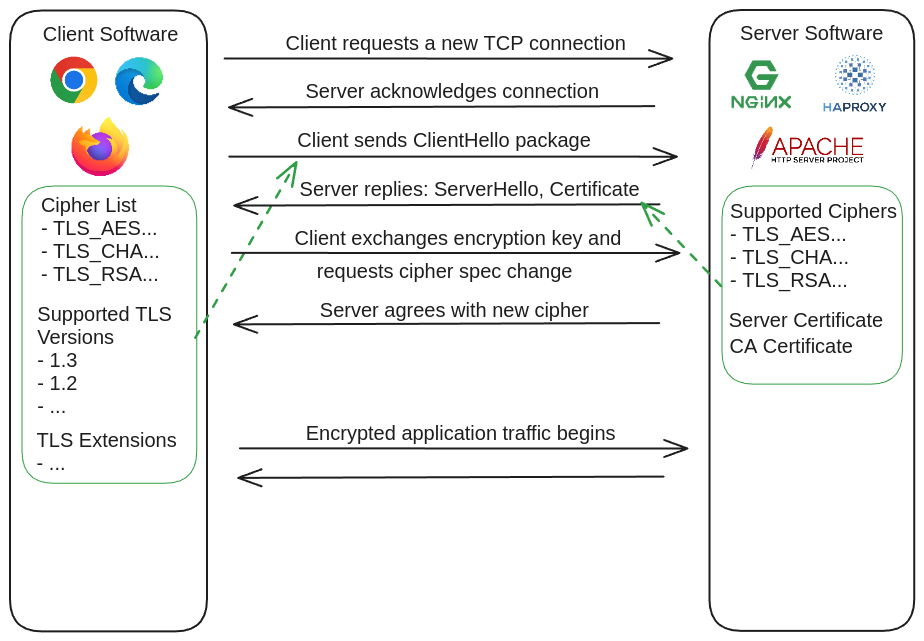
\includegraphics[height=10cm]{./images/tls_session.png}
    \caption{A TLS session between a web browser and a HTTPS server is created from a TCP connection}
\end{figure}

In general performing TLS fingerprinting on a client connection works by
analyzing the TLS ClientHello message that is sent by the client to the server
during the TLS handshake process.

\begin{figure}[!htb]
    \centering
    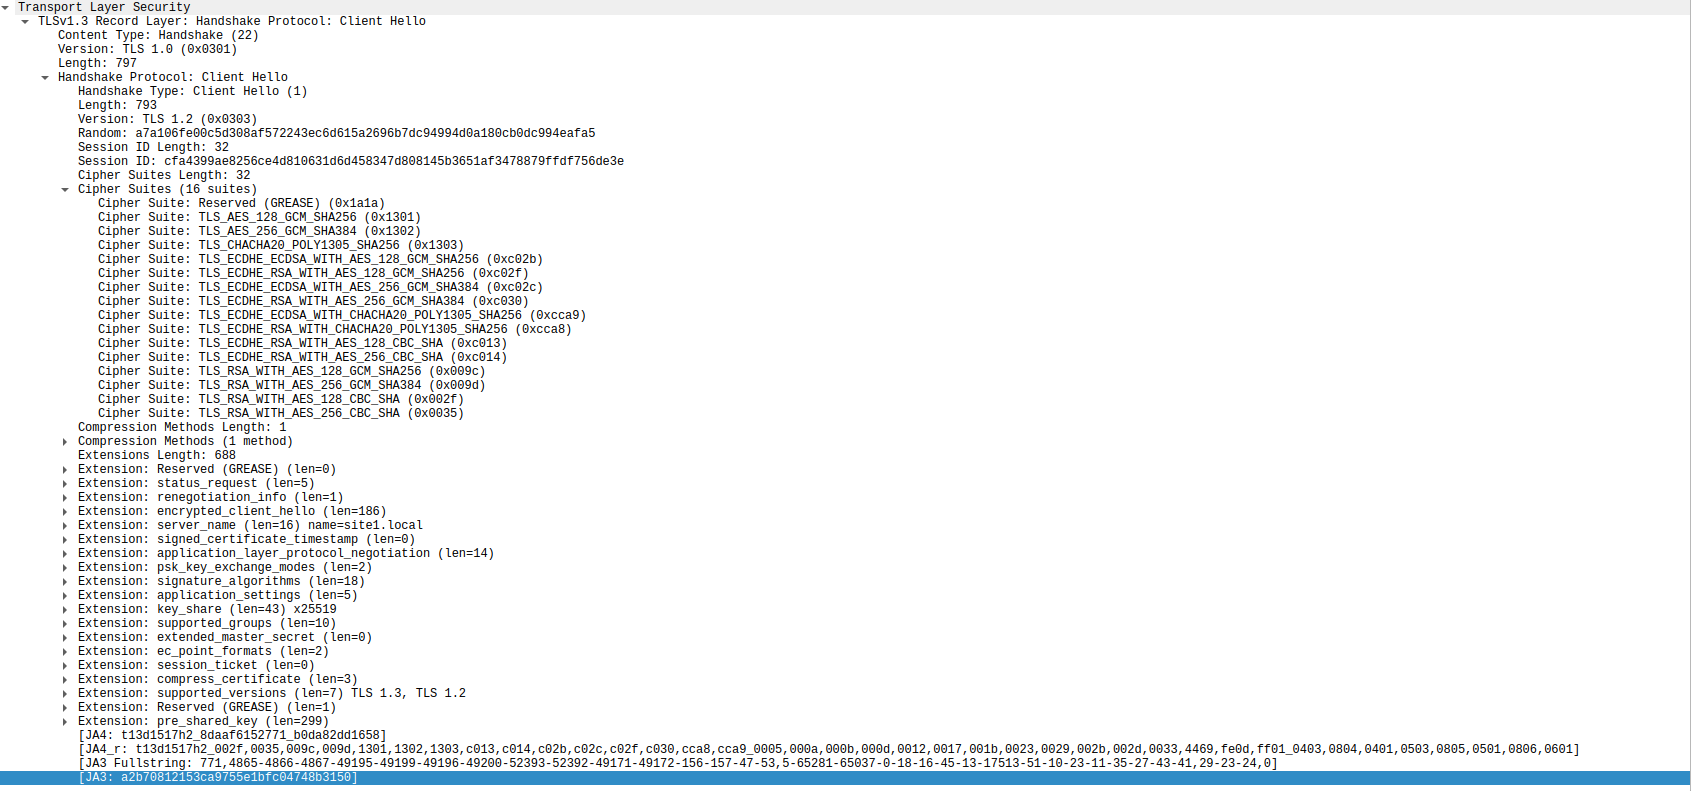
\includegraphics[height=7cm]{./images/tls_client_hello_wireshark.png}
    \caption{A TLS ClientHello packet captured using Wireshark}
\end{figure}

To generate a unique fingerprint out of this information several algorithms
already
exist.\\The JA3 algorithm proposed first by Salesforce \cite{ja3Salesforce}
collects values from the ClientHello into four different array lists and formats
them into one comma separated string that gets hashed. In detail the values used
from ClientHello are: SSLVersion, Cipher, SSLExtension, EllipticCurve,
EllipticCurvePointFormat.\\An example derived from a ClientHello looks like
this:
\begin{minted}[breaklines]{python}
"769,47-53-5-10-49161-49162-49171-49172-50-56-19-4,0-10-11,23-24-25,0"
\end{minted}
If no SSL extensions are used the field will be left empty. Example:
\begin{minted}[breaklines]{python}
"769,4-5-10-9-100-98-3-6-19-18-99,,,"
\end{minted}
To generate a unique identifier from this text the MD5 hash function is used.
It will leave us with the following 32 characters:
"ada70206e40642a3e4461f35503241d5". JA3 also needs to ignore values for non
existing extensions, because some TLS clients are using Google’s GREASE
(Generate Random Extensions And Sustain Extensibility). This is a feature
proposed by Google to break wrongly implemented TLS servers. It may sound
controversial at first, but comes with good intentions. In a internet draft
paper by D. Benjamin \cite{greaseDraft} he explains that its better to break
some production systems in place instead of risking flawed TLS
implementations to spread and risk outages of global scale.

JA3 seems to be
a good candidate for fingerprinting transparent phishing toolkits at first,
but it after some testing it comes clear that JA3 can not be used to
fingerprint instances of Google Chrome, due to it's reliance on the order of
the cipher extension list in the ClientHello package. Google chrome uses a
feature called "TLS ClientHello extension permutation" that prevents TLS
fingerprinting for said reason. This can be bypassed by sorting the numeric
values by size. Open source implementations of the JA3 algorithm with
normalized extension orders exist under the name "JA3N". Sadly in our
experimentation we were not able to reliably identify versions of Google
Chrome using JA3 for yet unkown reasons.
Luckily a better alternative
to the JA3 algorithm exists. The JA4+ family is a set of new network
fingerprinting algorithms developed by FoxIO \cite{foxIOJa4}. The JA4+
family also comes with a fingerprinting algorithm for TLS called JA4. JA4 is
superior to JA3 in many ways. It supports HTTP 3 including its UDP based
transport protocol QUIC and normalized the order of ciphers and extensions
by default. It uses a different output format than JA3 which consists of
three seperatable parts that more verbose and human readable in general. JA4
provides a more reliant and expressive fingerprinting solution for this
papers use case. Other open-source implementations of JA4 are avaible and
include a wireshark addon and an nginx fork. The later one will be used in
our lab setup to collect JA4 fingerprints.

\begin{figure}[!htb] \centering
	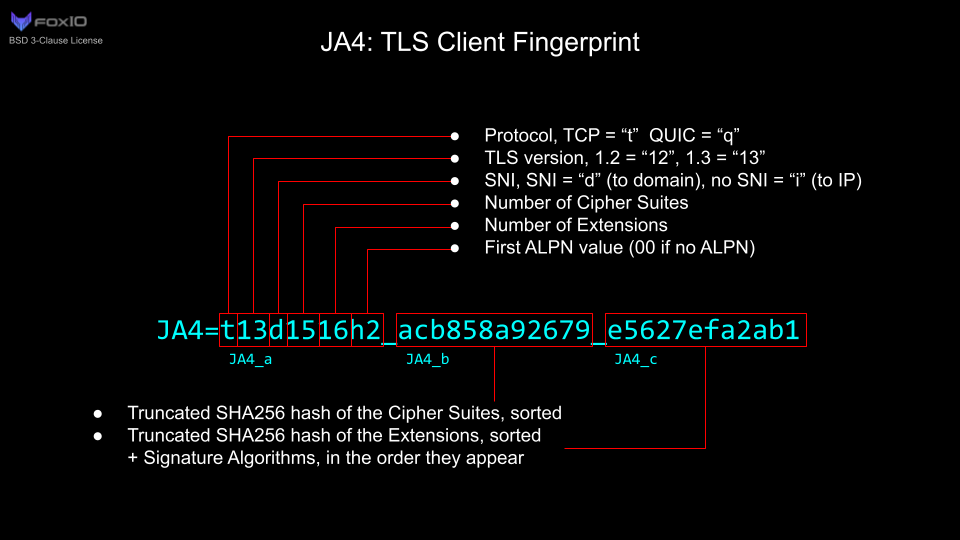
\includegraphics[height=7cm]{./images/JA4.png} \caption{JA4 TLS client
		fingerprint format} \end{figure}

\newpage
\section{Existing Countermeasures}
\subsection{Round Trip Time Analysis}
The round trip time (RTT) of a network connection is the time it takes for a
packet to travel from the sender to the receiver and back. It is an important
metric for measuring network performance and can be used to detect network
anomalies, such as packet loss or congestion.
In the context of this research RTT analysis can also be used to detect
the usage of reverse proxy software and MITM phishing toolkits.
In the previously mentioned paper by Kondracki the team was able to identify
the most common open-source MITM phishing toolkits by analyzing the RTT of
specific TCP handshake related packets. Because relaying traffic from a HTTPS
secured
web server, through the reverse proxy's own HTTPS server and then to the client,
there will be always two TCP connections for each client HTTP request.
This will lead to increased RTT values that can be measured.
In real world scenarios the delay added by physical and global routing factors,
will be
a hundred times larger than the delay added by a reverse proxy implementation.
To account for this the team measured the normal RTT of thousands of test
connections
across the globe. In their final statistical model this was enough to detect and
identify
the reverse proxy servers of transparent phishing toolkits with high reliability
based on their
TCP round trip timings alone.

\subsection{Mismatch of User-Agent and TLS Fingerprint} A broader and
more flexible approach then the previous blacklist solution which tries to
block or flag client requests using the TLS implementation of known
transparent phishing toolkits, is to focus on detecting requests from TLS
reverse proxies in general. The attack vector that is facilitate by abusing
reverse proxies to spy on a users TLS encrypted session is more commonly known
as a TLS MITM (Man in the Middle) Attack.\\The American content delivery
network operator Cloudflare which is also known for DDoS mitigation and other
cyber security related services is running an open-source monitoring service
called MALCOLM which stands for "Measuring Active Listeners, Connection
Observers, and Legitimate Monitors". It provides statistics about observed
HTTPS Interceptions. A HTTPS Interception defined in Cloudflare's own terms is
a request that comes from either a "A device has a root certificate installed
that allow an intermediary to decrypt and inspect traffic" or "An origin
server provides its TLS private key to a third party (like a reverse proxy)
that does TLS termination" \cite{cloudflareMALCOLM}. The second definition
means exactly the kind of TLS MITM attacks which we are trying to detect.\\The
monitoring platform is powered by "MITMEngine" (Monster-In-The-Middle Engine)
that Cloudflare describes as their HTTPS interception detector. MITMEngine is
an open-source software written in go. It works by matching TLS fingerprints
of requests to known browser User-Agent strings. If a mismatch is found the
request is marked as potentially crafted by HTTPS Interception. This strategy
again relies on maintaining a huge database of User-Agent and TLS Fingerprint
pairs. Cloudflare states on the MALCOLM dashboard website that they can only
identity 60\% of the clients that are served by their internal network.
Especially the detection of Android based devices is not reliably possible due
to the large amount of different Android based operating systems and browsers.
Readers of the MALCOLM website are encouraged to contribute User-Agent TLS
fingerprint pairs to the MITMEngine git repository to help overcome this
issue.


\newpage
\chapter{Experimentation}
\section{Simulation of Transparent Phishing Attacks}
To test and analyze the capabilities of the most popular open source
transparent phishing toolkits a controlled lab environment will be set up. The
goal is to find flaws in their attack implementation and to develop and test new
or improved countermeasures against these attacks.\\ First a web application
will be set up that is secured with a multi-factor authentication system. Then
the open source transparent phishing toolkits will be used to set up attack
simulations against this web application. The local web application will be
running on a local machine, but still be secured with a valid self-signed TLS
certificate. Our own certificate authority will have to be installed in the
browser used for testing, a recent version of google chrome in this case. In a
real world scenario an attacker would also have to buy a valid domain name. For
our simulated attacks an entry in the hosts fill be sufficient to redirect the
traffic to the local machine.\\ \begin{figure}[!htb] \centering
	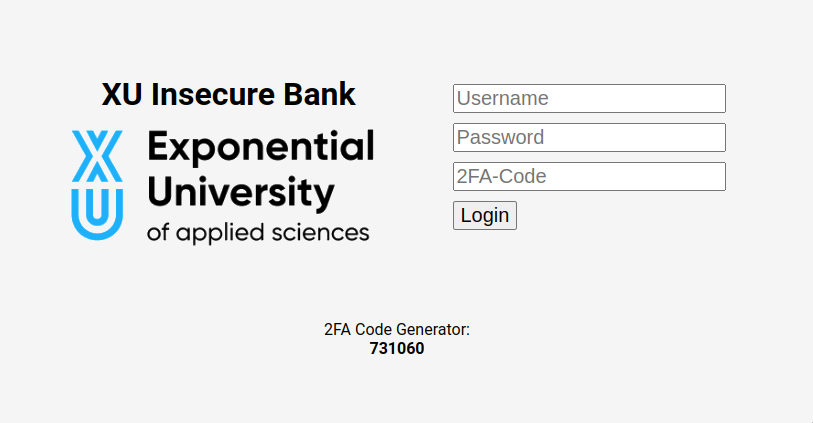
\includegraphics[height=7cm]{./images/2fa_app.png} \caption{Web application
		secured with a demo two-factor authentication system} \end{figure} The test
environment web application implements a very basic credential based login
system with two-factor authentication. For demo purposes the two-factor
authentication logic will accept any 6 digit number as valid token.\\The
frontend of this application is connected to a NodeJS based backend that is
using express.js for routing and parsing of incoming requests. After one
provides login credentials in the frontend a authentication endpoint in the
backend will be called with the provided credentials. If the credentials are
valid the backend will redirect the user to his profile page. This response will
also contain a session cookie that will be used to authenticate the user in the
future.\\For an attacker, stealing the content of that session cookie is enough
to gain full access to that account. This is also true for most real world web
applications where cookie based authenticaion is used, but this alone is not a
securiy issue. Nearly 99\% of all websites are TLS secured today
\cite{tlsPercentage} meaning that no one except the user and server can see the
content of that HTTP request including the session cookie.\\ \\

In our simulated attack scenario it will be our goal to steal the content of
this session cookie to overtake the victims session. In the real world an
attacker is likely saving login credentials eg. email and password from all
requests he intercepts with his transparent phsihing toolkit's mitm proxy.
Additionally he may inject custom HTML and JavaScript into the original page to
steal even more information from the victim using social engineering techniques,
for example by asking for an additional multi factor authentication token that
he can use in the future. For the purpose of this experiment we will only focus
on stealing the session cookie.\\ \\

\begin{figure}[!htb] \centering
	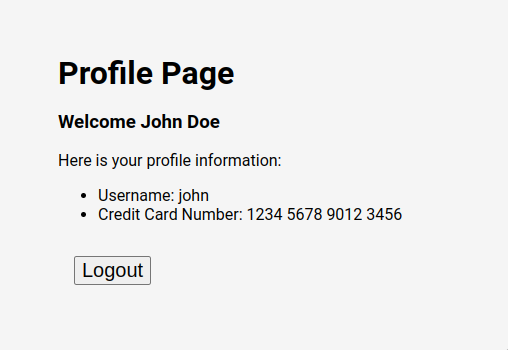
\includegraphics[height=7cm]{./images/profile_page.png} \caption{Profile page
		containing confidential information} \end{figure}

\newpage \section{Testing of Countermeasures} \subsection{Blacklisting well
	known TLS Fingerprints} The first countermeasure that we are trying to
implement
into our lab setup is to blacklist TLS fingerprints of well known
transparent phishing toolkits. This way we can detect if a client connection is
relayed through a transparent phishing toolkit and show the user a warning or
ignore the whole request. This approach comes with some obvious downsides:

\begin{itemize}
	\item The attacker can change the TLS fingerprint of his
	      transparent phishing toolkit by modifying the TLS stack of the toolkit or
	      by
	      using a different toolkit with an unknown fingerprint
	\item The attacker can spoof the TLS fingerprint of the victim's client
	\item The attacker downgrades to HTTP and does not use TLS at all
\end{itemize}

Following is an example implementation of a basic blocklist implemented using a
custom Nginx
fork that supports JA4 fingerprinting. If the client's TLS fingerprint is on the
blocklist, the request will be blocked and the client will receive a 403
Forbidden response. Instead of blocking the request, passing down information
about whether a malicious fingerprint was detected or not to the underlying
backend app, a HTTP header could be added.

\begin{minted}{nginx}
server {
     listen 443 ssl;
     server_name xu-bank.com;

     # ... other ssl configuration

     # blocklist
     map $http_ssl_ja4 $allowed_client {
         default                                 1;
         "t13d191000_9dc949149365_e7c285222651"  0; # evilginx2
     }

     location / {
         # block the request if the clients fingerprint is on the blocklist
         if($allowed_client = 0) {
             return 403;
         }

         # forward the request to the backend
         proxy_pass http://backend;
     }
}
\end{minted}

The same approach can be turned into a whitelist by inverting the logic. This
way only clients with a known good TLS fingerprint will be allowed to access the
web application. This approach is more secure, but also comes with the downside
that new clients will not be able to access the web application until their TLS
fingerprint is added to the whitelist. Maintaining a trusted JA4 fingerprint
database would require a lot of fingerprint collecting before said whitelist can
be used in production as many different browsers and TLS implementations exist
and change frequently.

\subsection{Validation of client cipher list} A TLS ClientHello packet sent
by a client always contains a list of supported ciphers. The list of ciphers
and its orders can be used to fingerprint the client. Many open-source MITM
reverse proxy solutions are already capable of spoofing the supported cipher
list in the ClientHello package. To detect client requests crafted by said
reverse
proxies more reliably, verifying the implementation of each cipher could be
helpful. A proof of concept cipher spoofing tool would need to support many
different ciphers. To overcome this issue using a TLS server stack that
supports as many ciphers as possible is required. In the cryptographic world
many battle tested
libaries exist that support a wide range of ciphers. The list includes OpenSSL,
GnuTLS, mbedTLS and BoringSSL.
As OpenSSL has a long history in development and adoption, it is a good
candidate for this task.
OpenSSL 3.1.1 supports 159 ciphers in the build that is shipped with Fedora39
Linux.

\begin{lstlisting}[breaklines=true,basicstyle=\tiny,caption={Listing supported
            ciphers and counting them in a shell},captionpos=b]
$ openssl ciphers -v 'ALL:eNULL'
TLS_AES_256_GCM_SHA384         TLSv1.3 Kx=any      Au=any   Enc=AESGCM(256)             Mac=AEAD
TLS_CHACHA20_POLY1305_SHA256   TLSv1.3 Kx=any      Au=any   Enc=CHACHA20/POLY1305(256)  Mac=AEAD
TLS_AES_128_GCM_SHA256         TLSv1.3 Kx=any      Au=any   Enc=AESGCM(128)             Mac=AEAD
TLS_AES_128_CCM_SHA256         TLSv1.3 Kx=any      Au=any   Enc=AESCCM(128)             Mac=AEAD
ECDHE-ECDSA-AES256-GCM-SHA384  TLSv1.2 Kx=ECDH     Au=ECDSA Enc=AESGCM(256)             Mac=AEAD
ECDHE-RSA-AES256-GCM-SHA384    TLSv1.2 Kx=ECDH     Au=RSA   Enc=AESGCM(256)             Mac=AEAD
DHE-DSS-AES256-GCM-SHA384      TLSv1.2 Kx=DH       Au=DSS   Enc=AESGCM(256)             Mac=AEAD
DHE-RSA-AES256-GCM-SHA384      TLSv1.2 Kx=DH       Au=RSA   Enc=AESGCM(256)             Mac=AEAD
ECDHE-ECDSA-CHACHA20-POLY1305  TLSv1.2 Kx=ECDH     Au=ECDSA Enc=CHACHA20/POLY1305(256)  Mac=AEAD
 ...
$ openssl ciphers -v 'ALL:eNULL' | wc -l # Count the number of ciphers
159
    \end{lstlisting}

OpenSSL may be more well known as a library for cryptographic functions, but it
also contains with a command line interface. The openssl binary comes with a
built-in TLS and HTTP server implementation called s\_server. It can be used to
quickly setup TLS servers for testing and debugging purposes. The list of
supported ciphers for a server can be configured using the -ciphers option for
TLSv1.2 and below and the -ciphersuites option for TLSv1.3 and above. For the
sake of this paper a proof of concept solution was implemented using a simple
bash script to spawn various instances of OpenSSL's s\_server with different
cipher configurations. To validate if a client actually supports his claimed
ciphers, each instance of s\_server will be configured to only support one
cipher. The client will then be forced to use this cipher to establish a
connection. If the client is not able to establish a connection an error will be
written to a log file that is supervised by our bash script.

\begin{minted}{bash}
...
# List of default ciphers supported by openssl s_server
ciphers=$(cat <<-END
TLSv1.3    :TLS_AES_128_GCM_SHA256
TLSv1.3    :TLS_AES_256_GCM_SHA384
...
END)

# Spawn static https server to serve check.html and api
www_port=8443
openssl s_server -key key.pem -cert cert.pem -accept $www_port -WWW 2>&1 &

# Start of test s_server port range
port=8000

while IFS= read -r line; do
cs=$(echo $line | sed 's/.*://')
echo "Spawning server with cipher: $cs"

cipher_param=""

# Detect if its TLSv1.3 or lower
is_tls13=$(echo $line | grep -c "TLSv1.3")

# Use the correct openssl command based on TLS version
if [ $is_tls13 -eq 1 ]; then
cipher_param="-ciphersuites $cs -no_tls1_2 -no_tls_1_1 -no_tls_1 -no_ssl3"
else
cipher_param="-cipher $cs -no_tls1_3"
fi

# Spawn s_server instance and redirect output log to file
openssl s_server -key key.pem -cert cert.pem -accept $port -www \
$cipher_param -debug >> "logs/$port-$cs.txt" 2>&1 &

port=$((port+1))
done <<< "$ciphers"

# Check all log files for errors and print overview of server status ...
\end{minted}

\newpage

Now the testing browser needs to connect to each of the spawned TLS sockets.
There are multiple ways to achieve this.
A "iframe" is a HTML element that allows web developers to embed other website
into the current page. Also it is possible
to use JavaScript's fetch API to create a connection, but the iframe approach is
more verbose as it directly shows
connection errors inside each iframe. To simplify the process of creating the
iframes a simple JavaScript script will be used:

\begin{minted}{javascript}
let framesDone = 0;
const onFrameDone = () => {
    framesDone++;
    if(framesDone === SERVER_AMOUNT){
        // Provide browser information to bash script & exit
        fetch(`https://${DOMAIN}:8444/`);
    }
}
const frames = document.getElementById('frames');
for(let i = 0; i < SERVER_AMOUNT; i++){
    const port = 8000+i;
    const url = `https://${DOMAIN}:${port}`;
    const frame = document.createElement('iframe');
    frame.src = url;
    frame.onload = onFrameDone;
    frame.onerror = onFrameDone;
    frames.appendChild(frame);
}
\end{minted}

After all iframes have either loaded successfully or failed the script performs
a final fetch request to another
s\_server that is running with the \-brief option. This server will collect the
clients User\-Agent and supported TLS ciphers.
After that, before the bash script exits, it will write a result JSON file that
contains information about each tested cipher including logs
of each s\_server instance that was used for cipher validation.

\begin{figure}
	\centering
	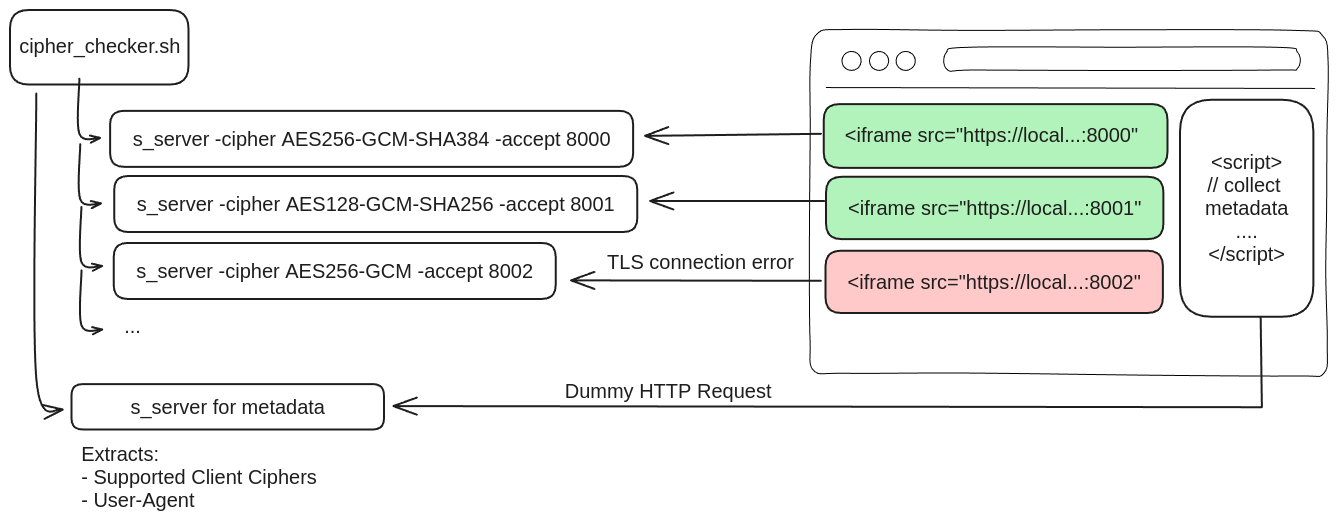
\includegraphics[height=5cm]{./images/cipher_check_setup.png}
	\caption{Using iframes to connect to all spawned s\_server instances}
\end{figure}

\newpage

To verify that this approach is working as expected across different versions of
browser
and TLS implementations a testing setup needed to be created.
As installing different versions of the same browser on the same machine is not
intended by the browser vendors and
some automated setup that is reasonably fast and reproducible is of interest, a
containerized setup was chosen.
Docker is the most popular containerization platform and is supported on all
major operating systems.
Due to the fact that this project is only intended for testing purposes and not
for production use, a more lightweight alternative
to Docker called Podman was used. It does not require root privileges to run
containers and is fully compatible with Docker images and containers.

\begin{figure}[!h]
	\centering
	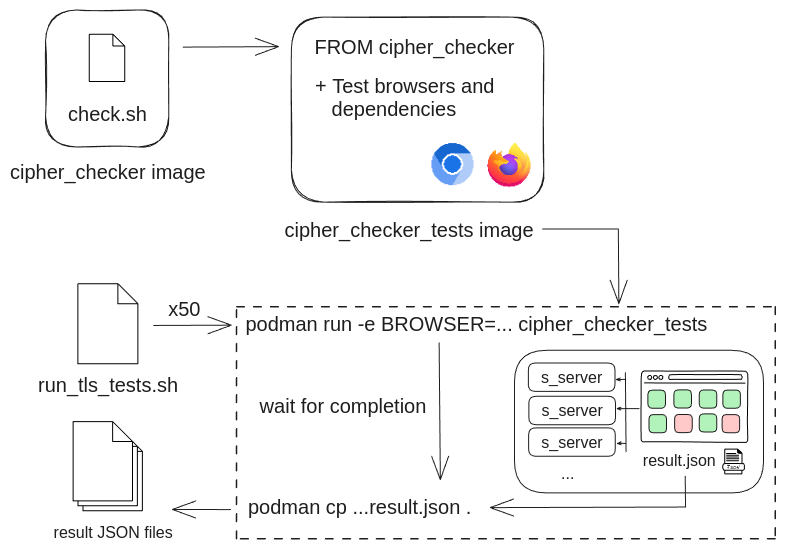
\includegraphics[height=10cm]{./images/cipher_checker_tests.png}
	\caption{The bash script spawns multiple instances of the
		cipher\_checker\_tests which includes check.sh and a browser for testing}
\end{figure}

To parse the result JSON files of each browser test, a python script was made.
It parses each JSON file, compares the supported ciphers
with the list of ciphers that the client told the server it supports and also
visualizes the results in a HTML table.
The resulting table shows all tested browser versions on the vertical axis and
all sent client ciphers on the other.

\newpage

\chapter{Results}
\section{Findings from Simulations}

\paragraph{Effectiveness of Toolkits}
The tested open-source transparent phishing toolkits were able to extract login credentials
and session cookies from the demo login site flawlessly. There was no visual difference in the relayed page
as expected. Using Evilginx2 was the most user-friendly experience, besides the fact that it requires the user
to create some special NS records to forward DNS queries to the Evilginx instance. Also it comes with many
configuration examples.

\paragraph{Detecting incoming relayed phishing traffic}
Detecting that an incoming HTTPS connection has been relayed reliably requires
analysis of many factors. Most importantly inspection of the TLS ClientHello packet
to fingerprint and verify the authenticity of the used client software.
Other factors like round trip time and TCP handshake timings can also be used to
detect MITM toolkit, but they require a large statistical model or usage of artificial intelligence.

\section{Proposed Solutions}
\paragraph{Detecting TLS cipher list spoofing}
To make the existing solutions that flag and or block incoming traffic that is likely
relayed through a reverse proxy of a transparent phishing toolkit, more reliable and harder
to circumvent, we proposed a proof of concept solution that enumerates all the received
client ciphers and checks if they are actually implemented.

\begin{figure}[!h]
    \centering
    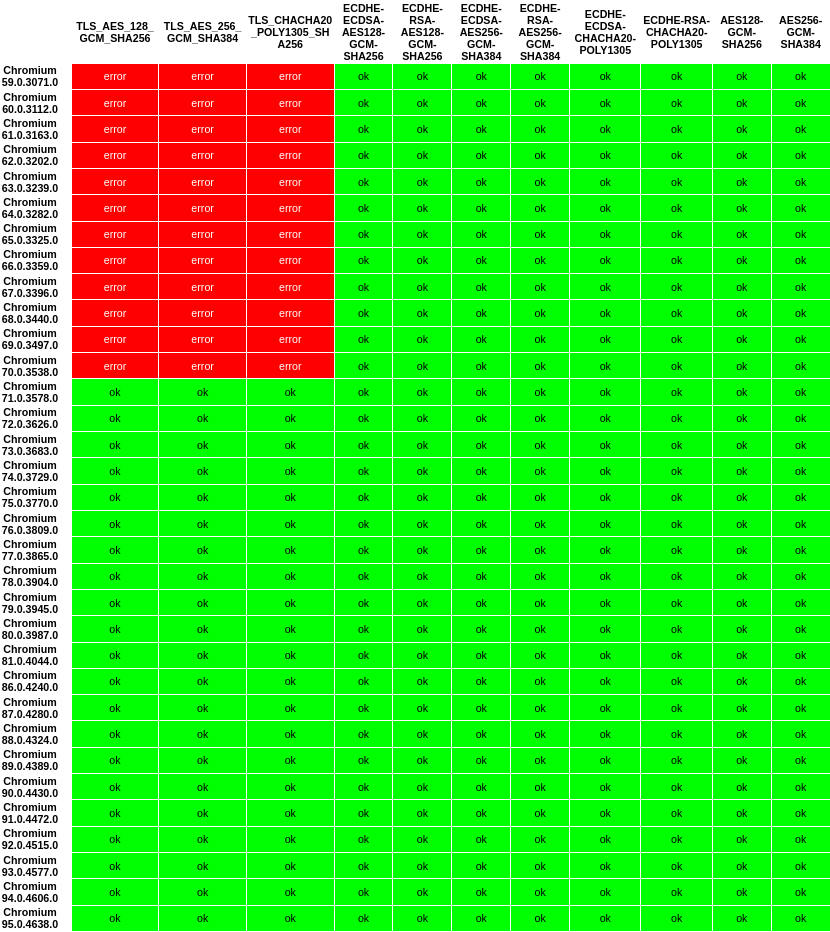
\includegraphics[height=18cm]{./images/cipher_checker_table.png}
    \caption{Cutoff results table screenshot of 56 different versions of the
        Chromium browser}
\end{figure}

\chapter{Discussion}
\section{Implications of Findings}

\paragraph{TLS client enumeration frameworks do not exist}
Besides that many TLS fingerprinting standards and implementations exist for clients,
all of them assume that the client's cipher list has not been altered. For TLS server on the other hand
a lot of open-source enumeration frameworks exist. These mostly focus on validating certificates and cipher implementations.
More of this is needed for web browsers and TLS clients in general.

\paragraph{Lack of TLS fingerprint database}
From literature and our own experimentation it comes clear that simple TLS fingerprinting
based detection methods, especially those which flag known malicious clients or whitelist
fingerprints of commonly used browsers, heavily rely on huge TLS fingerprint databases.
Creating and maintaining such a large dataset is a tedious task. It requires a vast user base
that is using different devices and browsers. Mobile users are way harder to fingerprint, due to the
variety that android based phones and browser apps come in. Also collecting TLS fingerprints and
performing TLS fingerprinting in general could rise some ethical concerns as it could be used
for user tracking or targeted advertisement.

\paragraph{Need for open-source browser testing framework}
While testing our proof of concept client cipher validation script we noticed that there is no
open-source browser testing project available that supports out of date versions of web browsers.
Browser testing and automation frameworks like Puppeteer or Playwright only support recent releases
of for example Google Chrome or Firefox. Download URLs of the browser binaries usually are hard coded
and pushed manually by the maintainer. Many commercial cloud based browser testing providers exist and
advertise that they support thousands of different browser products and versions, but in reality only support
the recent releases.

The findings from this research underscore the pressing need for enhanced detection mechanisms against transparent proxy phishing attacks. The implementation of advanced TLS fingerprinting techniques, such as JA4, demonstrates significant improvements over older methods, offering a more robust approach to identifying and mitigating these sophisticated threats. However, challenges remain in the areas of spoofing detection, user experience impact, and the necessity for comprehensive data collection.


\section{Limitations and Future Research}

\paragraph{Validation of client cipher list}
The proof of concept solution shell script check.sh was able to validate the
supported client ciphers of the 59 versions of chromium that we tested it with.
Unfortunately all of those tested browsers had the exact same client cipher list
which mean they use the same or a very similar TLS implementation. The client cipher list only
overlapped with 14 ciphers that our openssl s\_server based testing setup could
verify.

\paragraph{TLS fingerprinting vs large statistical models and AI}
This paper has shown that detecting transparent phishing relayed traffic by either
comparing the client TLS fingerprinting against known MITM phishing toolkits or normal browser fingerprints.
From there browsers can be either whitelisted or known phishing toolkits be blocked.
Other research, most importantly the paper "Catching Transparent Phish" by Brian Kondracki Et al. has shown
that with the usage of more detection factors and artificial intelligence a more reliable result can be achieved.
This comes at the price of higher complexity and the requirement of a even larger dataset.

This study identifies several limitations and avenues for future research in the quest to combat transparent proxy phishing attacks. The primary limitations include the reliance on a comprehensive TLS fingerprint database, the dynamic nature of TLS fingerprints, and the need for more sophisticated spoofing detection methods. The current lack of open-source tools for extensive browser testing further constrains the ability to validate detection mechanisms across a wide range of browser versions and configurations.

\newpage \bibliographystyle{plain} \bibliography{refs}

\end{document}